

\tikzset{every picture/.style={line width=0.75pt}} %set default line width to 0.75pt        

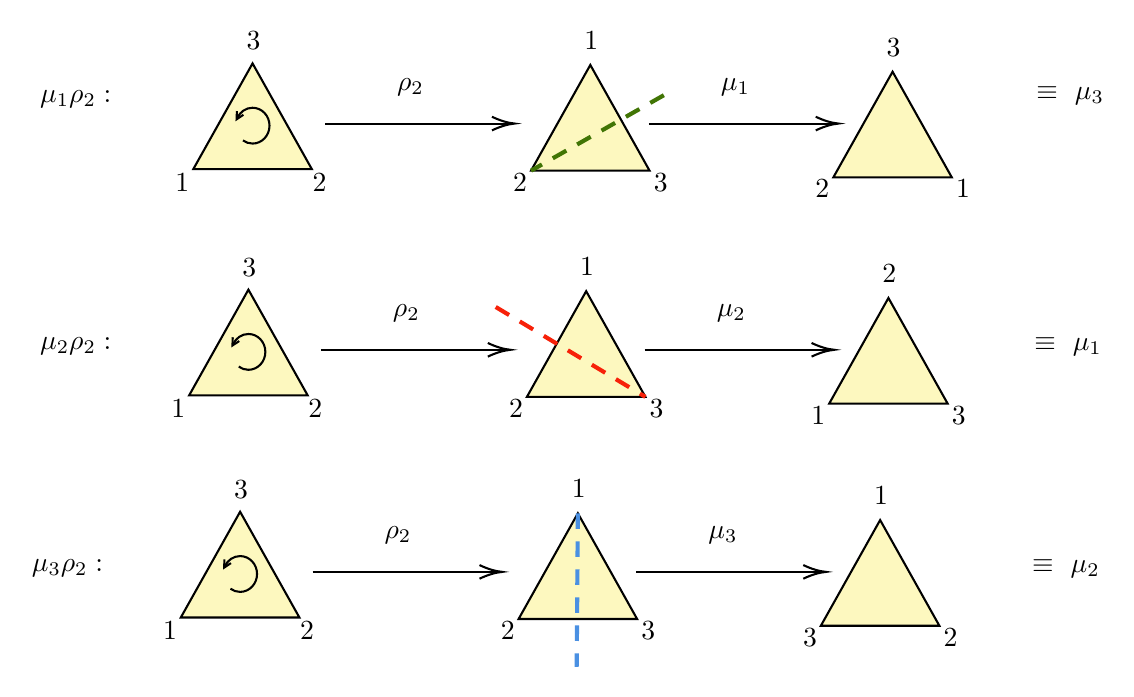
\begin{tikzpicture}[x=0.75pt,y=0.75pt,yscale=-1,xscale=1]
%uncomment if require: \path (0,336); %set diagram left start at 0, and has height of 336

%Shape: Triangle [id:dp7102908587227358] 
\draw  [fill={rgb, 255:red, 250; green, 238; blue, 106 }  ,fill opacity=0.43 ] (333.58,39.49) -- (362.13,90.43) -- (305.02,90.43) -- cycle ;

%Shape: Triangle [id:dp36216167148941303] 
\draw  [fill={rgb, 255:red, 250; green, 238; blue, 106 }  ,fill opacity=0.43 ] (170.85,38.75) -- (199.41,89.69) -- (142.29,89.69) -- cycle ;
%Straight Lines [id:da8658584840782982] 
\draw    (205.75,67.73) -- (295.12,67.73) ;
\draw [shift={(297.12,67.73)}, rotate = 180] [color={rgb, 255:red, 0; green, 0; blue, 0 }  ][line width=0.75]    (10.93,-3.29) .. controls (6.95,-1.4) and (3.31,-0.3) .. (0,0) .. controls (3.31,0.3) and (6.95,1.4) .. (10.93,3.29)   ;
%Shape: Arc [id:dp40227612494144915] 
\draw  [draw opacity=0] (163.49,65.01) .. controls (164.81,62.11) and (167.61,60.11) .. (170.85,60.11) .. controls (175.36,60.11) and (179.01,63.97) .. (179.01,68.74) .. controls (179.01,73.5) and (175.36,77.37) .. (170.85,77.37) .. controls (169.13,77.37) and (167.53,76.8) .. (166.21,75.84) -- (170.85,68.74) -- cycle ; \draw   (163.49,65.01) .. controls (164.81,62.11) and (167.61,60.11) .. (170.85,60.11) .. controls (175.36,60.11) and (179.01,63.97) .. (179.01,68.74) .. controls (179.01,73.5) and (175.36,77.37) .. (170.85,77.37) .. controls (169.13,77.37) and (167.53,76.8) .. (166.21,75.84) ;  
\draw   (166.43,63.51) -- (163.15,65.67) -- (163.31,61.69) ;

%Straight Lines [id:da418344717270963] 
\draw [color={rgb, 255:red, 65; green, 117; blue, 5 }  ,draw opacity=1 ][line width=1.5]  [dash pattern={on 5.63pt off 4.5pt}]  (369,54.07) -- (305.02,90.43) ;
%Shape: Triangle [id:dp4308225531048545] 
\draw  [fill={rgb, 255:red, 250; green, 238; blue, 106 }  ,fill opacity=0.43 ] (479.21,42.75) -- (507.76,93.69) -- (450.65,93.69) -- cycle ;

%Straight Lines [id:da6545411396067404] 
\draw    (361.75,67.73) -- (451.12,67.73) ;
\draw [shift={(453.12,67.73)}, rotate = 180] [color={rgb, 255:red, 0; green, 0; blue, 0 }  ][line width=0.75]    (10.93,-3.29) .. controls (6.95,-1.4) and (3.31,-0.3) .. (0,0) .. controls (3.31,0.3) and (6.95,1.4) .. (10.93,3.29)   ;
%Shape: Triangle [id:dp983539952898955] 
\draw  [fill={rgb, 255:red, 250; green, 238; blue, 106 }  ,fill opacity=0.43 ] (331.58,148.49) -- (360.13,199.43) -- (303.02,199.43) -- cycle ;

%Shape: Triangle [id:dp663497712579437] 
\draw  [fill={rgb, 255:red, 250; green, 238; blue, 106 }  ,fill opacity=0.43 ] (168.85,147.75) -- (197.41,198.69) -- (140.29,198.69) -- cycle ;
%Straight Lines [id:da3977158396253466] 
\draw    (203.75,176.73) -- (293.12,176.73) ;
\draw [shift={(295.12,176.73)}, rotate = 180] [color={rgb, 255:red, 0; green, 0; blue, 0 }  ][line width=0.75]    (10.93,-3.29) .. controls (6.95,-1.4) and (3.31,-0.3) .. (0,0) .. controls (3.31,0.3) and (6.95,1.4) .. (10.93,3.29)   ;
%Shape: Arc [id:dp8892762439816674] 
\draw  [draw opacity=0] (161.49,174.01) .. controls (162.81,171.11) and (165.61,169.11) .. (168.85,169.11) .. controls (173.36,169.11) and (177.01,172.97) .. (177.01,177.74) .. controls (177.01,182.5) and (173.36,186.37) .. (168.85,186.37) .. controls (167.13,186.37) and (165.53,185.8) .. (164.21,184.84) -- (168.85,177.74) -- cycle ; \draw   (161.49,174.01) .. controls (162.81,171.11) and (165.61,169.11) .. (168.85,169.11) .. controls (173.36,169.11) and (177.01,172.97) .. (177.01,177.74) .. controls (177.01,182.5) and (173.36,186.37) .. (168.85,186.37) .. controls (167.13,186.37) and (165.53,185.8) .. (164.21,184.84) ;  
\draw   (164.43,172.51) -- (161.15,174.67) -- (161.31,170.69) ;

%Shape: Triangle [id:dp32239079403343107] 
\draw  [fill={rgb, 255:red, 250; green, 238; blue, 106 }  ,fill opacity=0.43 ] (477.21,151.75) -- (505.76,202.69) -- (448.65,202.69) -- cycle ;

%Straight Lines [id:da052722364870694594] 
\draw    (359.75,176.73) -- (449.12,176.73) ;
\draw [shift={(451.12,176.73)}, rotate = 180] [color={rgb, 255:red, 0; green, 0; blue, 0 }  ][line width=0.75]    (10.93,-3.29) .. controls (6.95,-1.4) and (3.31,-0.3) .. (0,0) .. controls (3.31,0.3) and (6.95,1.4) .. (10.93,3.29)   ;
%Straight Lines [id:da8686264965245885] 
\draw [color={rgb, 255:red, 247; green, 33; blue, 9 }  ,draw opacity=1 ][line width=1.5]  [dash pattern={on 5.63pt off 4.5pt}]  (288,156.1) -- (360.13,199.43) ;
%Shape: Triangle [id:dp3646928922959751] 
\draw  [fill={rgb, 255:red, 250; green, 238; blue, 106 }  ,fill opacity=0.43 ] (327.58,255.49) -- (356.13,306.43) -- (299.02,306.43) -- cycle ;

%Shape: Triangle [id:dp06252827565832642] 
\draw  [fill={rgb, 255:red, 250; green, 238; blue, 106 }  ,fill opacity=0.43 ] (164.85,254.75) -- (193.41,305.69) -- (136.29,305.69) -- cycle ;
%Straight Lines [id:da9493236769564709] 
\draw    (199.75,283.73) -- (289.12,283.73) ;
\draw [shift={(291.12,283.73)}, rotate = 180] [color={rgb, 255:red, 0; green, 0; blue, 0 }  ][line width=0.75]    (10.93,-3.29) .. controls (6.95,-1.4) and (3.31,-0.3) .. (0,0) .. controls (3.31,0.3) and (6.95,1.4) .. (10.93,3.29)   ;
%Shape: Arc [id:dp8143767822487923] 
\draw  [draw opacity=0] (157.49,281.01) .. controls (158.81,278.11) and (161.61,276.11) .. (164.85,276.11) .. controls (169.36,276.11) and (173.01,279.97) .. (173.01,284.74) .. controls (173.01,289.5) and (169.36,293.37) .. (164.85,293.37) .. controls (163.13,293.37) and (161.53,292.8) .. (160.21,291.84) -- (164.85,284.74) -- cycle ; \draw   (157.49,281.01) .. controls (158.81,278.11) and (161.61,276.11) .. (164.85,276.11) .. controls (169.36,276.11) and (173.01,279.97) .. (173.01,284.74) .. controls (173.01,289.5) and (169.36,293.37) .. (164.85,293.37) .. controls (163.13,293.37) and (161.53,292.8) .. (160.21,291.84) ;  
\draw   (160.43,279.51) -- (157.15,281.67) -- (157.31,277.69) ;

%Shape: Triangle [id:dp83267999664511] 
\draw  [fill={rgb, 255:red, 250; green, 238; blue, 106 }  ,fill opacity=0.43 ] (473.21,258.75) -- (501.76,309.69) -- (444.65,309.69) -- cycle ;

%Straight Lines [id:da5336259749775443] 
\draw    (355.75,283.73) -- (445.12,283.73) ;
\draw [shift={(447.12,283.73)}, rotate = 180] [color={rgb, 255:red, 0; green, 0; blue, 0 }  ][line width=0.75]    (10.93,-3.29) .. controls (6.95,-1.4) and (3.31,-0.3) .. (0,0) .. controls (3.31,0.3) and (6.95,1.4) .. (10.93,3.29)   ;
%Straight Lines [id:da8799338674484278] 
\draw [color={rgb, 255:red, 74; green, 144; blue, 226 }  ,draw opacity=1 ][line width=1.5]  [dash pattern={on 5.63pt off 4.5pt}]  (327.58,255.49) -- (327,329.52) ;

% Text Node
\draw (132.22,90.31) node [anchor=north west][inner sep=0.75pt]    {$1$};
% Text Node
\draw (198.3,90.31) node [anchor=north west][inner sep=0.75pt]    {$2$};
% Text Node
\draw (166.48,22.11) node [anchor=north west][inner sep=0.75pt]    {$3$};
% Text Node
\draw (239,44.4) node [anchor=north west][inner sep=0.75pt]    {$\rho _{2}$};
% Text Node
\draw (395,44.4) node [anchor=north west][inner sep=0.75pt]    {$\mu _{1}$};
% Text Node
\draw (547,48.4) node [anchor=north west][inner sep=0.75pt]    {$\equiv \ \mu _{3}$};
% Text Node
\draw (130.22,199.31) node [anchor=north west][inner sep=0.75pt]    {$1$};
% Text Node
\draw (196.3,199.31) node [anchor=north west][inner sep=0.75pt]    {$2$};
% Text Node
\draw (164.48,131.11) node [anchor=north west][inner sep=0.75pt]    {$3$};
% Text Node
\draw (237,153.4) node [anchor=north west][inner sep=0.75pt]    {$\rho _{2}$};
% Text Node
\draw (393,153.4) node [anchor=north west][inner sep=0.75pt]    {$\mu _{2}$};
% Text Node
\draw (546,169.4) node [anchor=north west][inner sep=0.75pt]    {$\equiv \ \mu _{1}$};
% Text Node
\draw (67,50.12) node [anchor=north west][inner sep=0.75pt]    {$\mu _{1} \rho _{2} :$};
% Text Node
\draw (67,169.12) node [anchor=north west][inner sep=0.75pt]    {$\mu _{2} \rho _{2} :$};
% Text Node
\draw (126.22,306.31) node [anchor=north west][inner sep=0.75pt]    {$1$};
% Text Node
\draw (192.3,306.31) node [anchor=north west][inner sep=0.75pt]    {$2$};
% Text Node
\draw (160.48,238.11) node [anchor=north west][inner sep=0.75pt]    {$3$};
% Text Node
\draw (233,260.4) node [anchor=north west][inner sep=0.75pt]    {$\rho _{2}$};
% Text Node
\draw (389,260.4) node [anchor=north west][inner sep=0.75pt]    {$\mu _{3}$};
% Text Node
\draw (545,276.4) node [anchor=north west][inner sep=0.75pt]    {$\equiv \ \mu _{2}$};
% Text Node
\draw (63,276.12) node [anchor=north west][inner sep=0.75pt]    {$\mu _{3} \rho _{2} :$};
% Text Node
\draw (468.84,241.29) node [anchor=north west][inner sep=0.75pt]    {$1$};
% Text Node
\draw (502.29,309.49) node [anchor=north west][inner sep=0.75pt]    {$2$};
% Text Node
\draw (434.57,309.49) node [anchor=north west][inner sep=0.75pt]    {$3$};
% Text Node
\draw (323.21,238.03) node [anchor=north west][inner sep=0.75pt]    {$1$};
% Text Node
\draw (356.66,306.23) node [anchor=north west][inner sep=0.75pt]    {$3$};
% Text Node
\draw (288.94,306.23) node [anchor=north west][inner sep=0.75pt]    {$2$};
% Text Node
\draw (472.84,134.29) node [anchor=north west][inner sep=0.75pt]    {$2$};
% Text Node
\draw (506.29,202.49) node [anchor=north west][inner sep=0.75pt]    {$3$};
% Text Node
\draw (438.57,202.49) node [anchor=north west][inner sep=0.75pt]    {$1$};
% Text Node
\draw (327.21,131.03) node [anchor=north west][inner sep=0.75pt]    {$1$};
% Text Node
\draw (360.66,199.23) node [anchor=north west][inner sep=0.75pt]    {$3$};
% Text Node
\draw (292.94,199.23) node [anchor=north west][inner sep=0.75pt]    {$2$};
% Text Node
\draw (474.84,25.29) node [anchor=north west][inner sep=0.75pt]    {$3$};
% Text Node
\draw (508.29,93.49) node [anchor=north west][inner sep=0.75pt]    {$1$};
% Text Node
\draw (440.57,93.49) node [anchor=north west][inner sep=0.75pt]    {$2$};
% Text Node
\draw (329.21,22.03) node [anchor=north west][inner sep=0.75pt]    {$1$};
% Text Node
\draw (362.66,90.23) node [anchor=north west][inner sep=0.75pt]    {$3$};
% Text Node
\draw (294.94,90.23) node [anchor=north west][inner sep=0.75pt]    {$2$};


\end{tikzpicture}
